\documentclass[12pt,a4paper]{article}

% --- Packages ---
\usepackage[utf8]{inputenc}
\usepackage[margin=1in]{geometry}
\usepackage{amsmath,amssymb,amsfonts}
\usepackage{booktabs}
\usepackage{tabularx}
\usepackage{enumitem}
\usepackage{hyperref}
\usepackage{tikz}
\usetikzlibrary{shapes.geometric, arrows.meta, positioning, fit, backgrounds}

% --- TikZ Style ---
\tikzset{
    block/.style={rectangle, draw=black, fill=white, text centered, minimum height=2.2em, minimum width=4cm, font=\small, inner sep=5pt},
    arrow/.style={thick, ->, >=stealth}
}

% --- Document Info ---
\title{\textbf{\LARGE EduTwin – AI Digital Twin for Education}\\[0.4em]
\large Personalized Study Coach and Career Mentor}
\author{}
\date{}

\begin{document}

\maketitle

\section*{Abstract}
EduTwin is an AI-powered Digital Twin system designed to provide personalized educational guidance by maintaining a continuously evolving representation of a learner. Unlike conventional AI assistants that primarily rely on the current conversation and provide relatively stateless responses, EduTwin maintains structured information about the learner, including their profile, goals, preferences, knowledge, skills, interests, and relevant long-term memories.

The project investigates whether a continuously updated Digital Twin can improve the personalization, relevance, and consistency of AI-assisted educational interactions. The system combines large language models, structured learner modeling, long-term memory, semantic retrieval, recommendation mechanisms, prediction capabilities, explainability, and an interactive web-based interface.

The architecture separates the learner's current state from historical interaction evidence. The Digital Twin represents the system's current beliefs about the learner, while the Memory System preserves historical evidence that can later be retrieved to support updates and personalized responses. This separation allows the learner model to evolve without requiring the Twin itself to store an entire interaction history.

The final system provides a unified AI interaction experience through a modern web interface. Rather than requiring the learner to manually select a specialized AI agent, the system is designed around a single conversational interface in which the user's intent determines which internal capabilities should be activated.

The project was developed as a collaborative research and engineering effort covering AI architecture, learner modeling, memory systems, retrieval, recommendation, prediction, explainability, knowledge representation, AI agents, backend services, and frontend development.

\newpage

\section{Introduction}

\subsection{Background}
Artificial intelligence has increasingly become part of modern education, particularly through conversational systems capable of answering questions, explaining concepts, generating study material, and providing recommendations.

However, many existing AI assistants operate primarily on the information available within the current interaction. Although conversation history can provide some continuity, a conventional conversational model does not necessarily maintain an explicit and structured representation of the learner.

This creates an important limitation in educational personalization.

For example, an AI system may know that a student is currently asking about machine learning, but it may not explicitly represent:
\begin{itemize}[noitemsep,topsep=2pt]
    \item the student's existing knowledge of machine learning;
    \item their confidence in a particular skill;
    \item their long-term career goals;
    \item their preferred learning methods;
    \item their interests;
    \item topics they have previously struggled with;
    \item previous evidence that should influence future recommendations.
\end{itemize}

EduTwin addresses this problem by introducing a Digital Twin of the learner.

\subsection{Project Motivation}
The main motivation behind EduTwin is to investigate whether an AI system can provide more meaningful personalization when it maintains a continuously evolving learner model.

Instead of treating every interaction independently, EduTwin attempts to maintain a persistent representation of the student and update it as new evidence becomes available.

The system therefore moves from:
\begin{center}
    User $\rightarrow$ Question $\rightarrow$ AI Response
\end{center}
towards:
\begin{center}
    User $\rightarrow$ Interaction $\rightarrow$ Evidence $\rightarrow$ Memory $\rightarrow$ Twin Update $\rightarrow$ Personalized AI Response
\end{center}

This architecture allows the system to use both the learner's current state and relevant historical evidence when producing future responses.

\section{Research Question}
The central research question of the project is:

\begin{quote}
\textbf{Can a continuously evolving Digital Twin improve personalization compared with a stateless AI assistant?}
\end{quote}

To investigate this question, the project explores how different components can work together to create a persistent and adaptive learner representation.

The major research areas include:
\begin{itemize}[noitemsep,topsep=2pt]
    \item Digital Twin architectures;
    \item user modeling;
    \item long-term memory;
    \item semantic retrieval;
    \item knowledge representation;
    \item personalization;
    \item recommendation systems;
    \item prediction;
    \item explainable AI;
    \item LLM-based agents.
\end{itemize}

\section{Project Objectives}
The main objectives of EduTwin were:
\begin{enumerate}[noitemsep,topsep=2pt]
    \item Develop a structured Digital Twin representation of a learner.
    \item Store important learner characteristics in a machine-readable format.
    \item Maintain long-term memories from meaningful interactions.
    \item Retrieve relevant historical evidence when required.
    \item Continuously update the learner model using new evidence.
    \item Provide personalized educational recommendations.
    \item Support study coaching and career guidance.
    \item Provide predictive capabilities based on the learner's current state and evidence.
    \item Provide explanations for recommendations and system decisions.
    \item Integrate the different AI capabilities behind a unified conversational interface.
    \item Develop an interactive visualization of the learner's knowledge representation.
    \item Create a modern web-based GUI rather than a simple research prototype.
    \item Design the architecture so that the system can later be extended with more advanced databases, agents, and personalization mechanisms.
\end{enumerate}

\section{System Overview}
EduTwin consists of several interconnected components.

At a high level, the system can be represented as:

\begin{figure}[htbp]
\centering
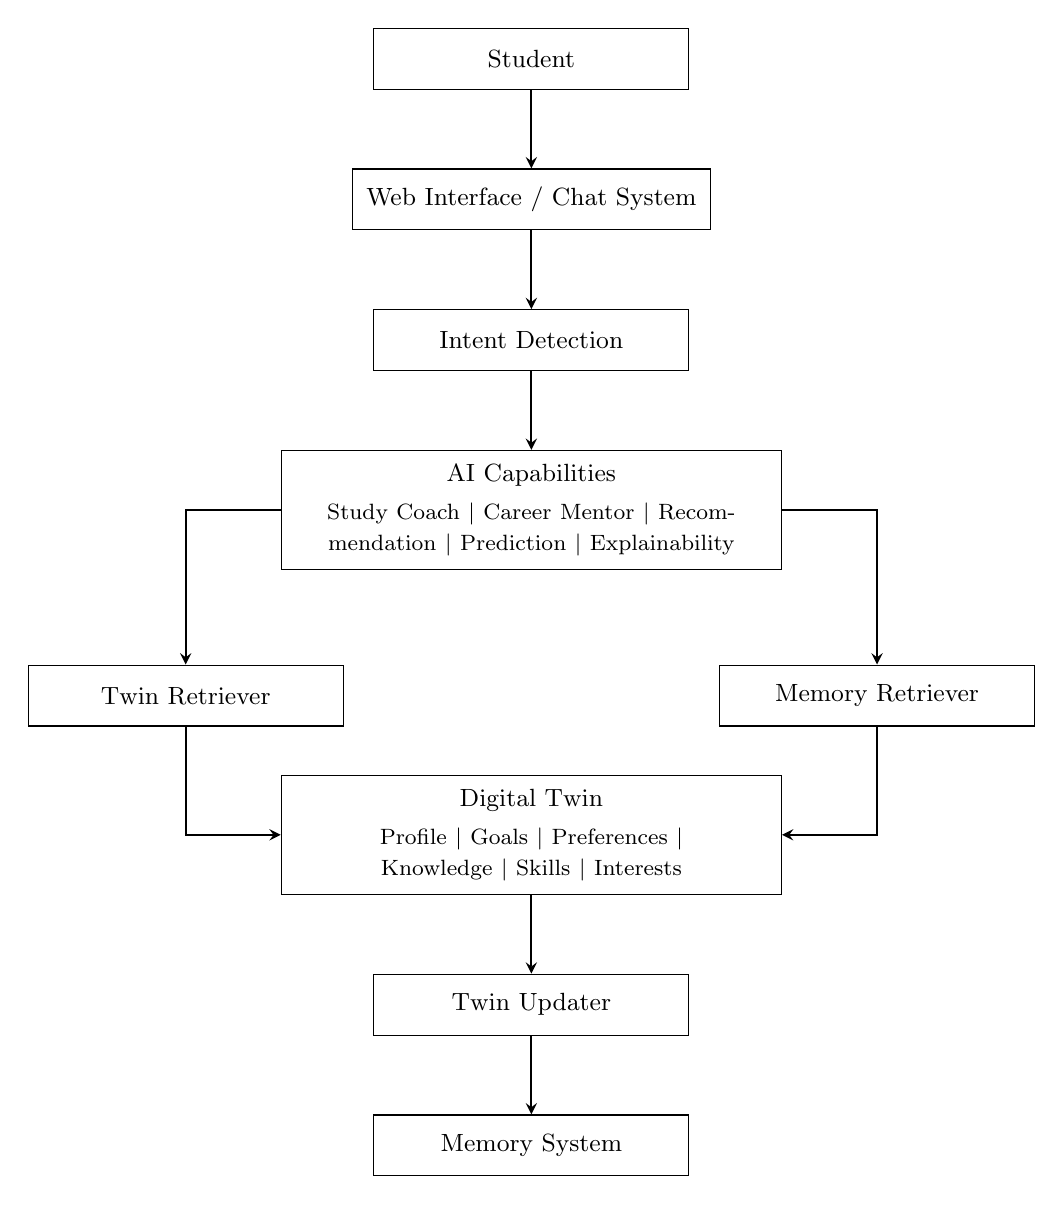
\begin{tikzpicture}[node distance=1cm, auto]
    \node (student) [block] {Student};
    \node (web) [block, below=of student] {Web Interface / Chat System};
    \node (intent) [block, below=of web] {Intent Detection};
    \node (ai) [block, below=of intent, text width=6cm] {AI Capabilities\\[0.3em] \footnotesize Study Coach $\mid$ Career Mentor $\mid$ Recommendation $\mid$ Prediction $\mid$ Explainability};
    
    \node (twin_ret) [block, below left=1.2cm and -0.8cm of ai, text width=3.2cm] {Twin Retriever};
    \node (mem_ret) [block, below right=1.2cm and -0.8cm of ai, text width=3.2cm] {Memory Retriever};
    
    \node (twin) [block, below=2.6cm of ai, text width=6cm] {Digital Twin\\[0.3em] \footnotesize Profile $\mid$ Goals $\mid$ Preferences $\mid$ Knowledge $\mid$ Skills $\mid$ Interests};
    \node (updater) [block, below=of twin] {Twin Updater};
    \node (mem_sys) [block, below=of updater] {Memory System};

    \draw [arrow] (student) -- (web);
    \draw [arrow] (web) -- (intent);
    \draw [arrow] (intent) -- (ai);
    \draw [arrow] (ai) -| (twin_ret);
    \draw [arrow] (ai) -| (mem_ret);
    \draw [arrow] (twin_ret) |- (twin);
    \draw [arrow] (mem_ret) |- (twin);
    \draw [arrow] (twin) -- (updater);
    \draw [arrow] (updater) -- (mem_sys);
\end{tikzpicture}
\caption{System Overview Diagram.}
\end{figure}

The architecture was designed so that the Digital Twin represents the current learner state, while the Memory System represents historical evidence.

\section{Digital Twin Architecture}

\subsection{Learner Representation}
The Digital Twin acts as a structured representation of the learner.

It contains multiple components:
\begin{itemize}[noitemsep,topsep=2pt]
    \item Profile
    \item Goals
    \item Preferences
    \item Knowledge
    \item Skills
    \item Interests
    \item Memories
    \item Student aggregation model
\end{itemize}

The purpose of separating these components is to allow different types of learner information to be represented independently while still being combined into a single learner model.

\subsection{Student Model}
The Student model acts as an aggregate of the different Digital Twin components.

Conceptually:

\begin{itemize}[noitemsep,topsep=2pt]
    \item[] \textbf{Student}
    \begin{itemize}[noitemsep,topsep=1pt]
        \item[$\vdash$] Profile
        \item[$\vdash$] Goals
        \item[$\vdash$] Preferences
        \item[$\vdash$] Knowledge
        \item[$\vdash$] Skills
        \item[$\vdash$] Interests
        \item[$\llcorner$] Memories / Evidence
    \end{itemize}
\end{itemize}

This provides a centralized representation that can be accessed by the different AI capabilities.

\section{Profile Modeling}
The Profile component represents relatively stable information about the learner.

Examples include:
\begin{itemize}[noitemsep,topsep=2pt]
    \item educational background;
    \item academic information;
    \item general learner characteristics;
    \item relevant personal information required for personalization.
\end{itemize}

The profile is intended to provide contextual information without requiring the system to reconstruct it from historical conversations.

\section{Goal Modeling}
Goals represent the objectives that the learner is attempting to achieve.

Goals can be used to personalize:
\begin{itemize}[noitemsep,topsep=2pt]
    \item learning recommendations;
    \item study plans;
    \item career guidance;
    \item skill development;
    \item learning priorities.
\end{itemize}

For example, if a learner's goal is to become an AI engineer, recommendations can be evaluated according to their relevance to that long-term objective.

\section{Preference Modeling}
The preference system was designed to represent learner preferences using affinity belief vectors.

Rather than treating preferences as simple binary values, the system can represent the degree to which the learner is believed to prefer a particular option.

This creates a more flexible representation of uncertain preferences.

The preference representation can therefore evolve as new evidence is collected.

For example:
\begin{itemize}[noitemsep,topsep=2pt]
    \item[] \textbf{Preference}
    \begin{itemize}[noitemsep,topsep=1pt]
        \item[$\vdash$] Topic affinity
        \item[$\vdash$] Learning-method affinity
        \item[$\vdash$] Content affinity
        \item[$\llcorner$] Other preference dimensions
    \end{itemize}
\end{itemize}

The system can update these beliefs when new interaction evidence provides support for or against an existing preference.

\section{Knowledge Modeling}
The Knowledge component represents the system's current belief about what the learner knows.

Each knowledge item contains information such as:
\begin{itemize}[noitemsep,topsep=2pt]
    \item \texttt{knowledge\_id}
    \item \texttt{topic}
    \item \texttt{mastery}
\end{itemize}

Mastery represents the system's estimated level of understanding of a particular topic.

An important architectural decision was that the Knowledge component stores the current belief state, rather than storing every historical change.

For example:
\begin{quote}
\textbf{Machine Learning}\\
\textbf{Mastery:} 0.72
\end{quote}

The fact that mastery previously had a value of 0.50 is not stored directly inside the current Twin state.

Instead, historical evidence is maintained through the Memory System.

This keeps the Digital Twin compact and separates current beliefs from historical evidence.

\section{Skill Modeling}
Skills follow a similar principle but represent practical or capability-oriented competencies.

Each Skill contains:
\begin{itemize}[noitemsep,topsep=2pt]
    \item \texttt{skill\_id}
    \item \texttt{name}
    \item \texttt{skill\_level}
    \item \texttt{confidence}
    \item \texttt{last\_updated}
\end{itemize}

Both \texttt{skill\_level} and \texttt{confidence} are represented numerically between 0 and 1.

This distinction is important because the system may have:
\begin{itemize}[noitemsep,topsep=2pt]
    \item high confidence that the learner has a particular skill;
    \item but only moderate evidence for the actual skill level.
\end{itemize}

The \texttt{last\_updated} field also provides temporal context for the current belief.

\section{Memory System}
One of the major components developed during the project was the long-term Memory System.

The purpose of the Memory System is to preserve useful evidence from interactions that may become relevant later.

The system does not attempt to store every message as a permanent learner fact.

Instead, it determines whether information from an interaction is worth remembering.

The resulting architecture is:
\begin{center}
\textbf{Interaction} $\rightarrow$ \textbf{Rule Filter} $\rightarrow$ \textbf{LLM Memory Decision} $\rightarrow$ \textbf{Memory Object} $\rightarrow$ \textbf{Memory Store} $\rightarrow$ \textbf{Vector Database}
\end{center}

\section{Memory Decision Pipeline}
A rule-based filtering stage is first used to determine whether an interaction is potentially meaningful.

This prevents every interaction from automatically becoming long-term memory.

For interactions that pass the initial filtering stage, an LLM-based structured decision process is used.

The model determines whether the information should become a memory and, where appropriate, produces a structured memory representation.

This creates a controlled pipeline rather than blindly storing the entire conversation.

\section{Memory Representation}
The Memory model was implemented as a structured object.

A memory can contain information such as:
\begin{itemize}[noitemsep,topsep=2pt]
    \item memory content;
    \item importance;
    \item timestamp;
    \item relevance;
    \item affected Digital Twin components;
    \item associated metadata.
\end{itemize}

The system therefore transforms unstructured conversational information into structured evidence that can later be retrieved.

\section{ChromaDB Memory Store}
The implemented Memory Store uses ChromaDB as the vector database.

Embeddings are generated within the Memory Store, allowing memories to be represented in vector space.

This enables semantic retrieval rather than relying only on exact keyword matching.

The resulting architecture is approximately:
\begin{itemize}[noitemsep,topsep=2pt]
    \item[] \textbf{Memory}
    \begin{itemize}[noitemsep,topsep=1pt]
        \item[$\vdash$] Content
        \item[$\vdash$] Metadata
        \item[$\llcorner$] Embedding $\longrightarrow$ \textbf{ChromaDB}
    \end{itemize}
\end{itemize}

The Memory Store also includes duplicate detection to reduce unnecessary repetition of memories.

\section{Memory Retrieval}
A dedicated \texttt{MemoryRetriever} was developed to retrieve historical evidence relevant to the current interaction.

The retrieval process is based on semantic relevance while also considering additional properties of memories.

The proposed ranking mechanism combines:
\begin{itemize}[noitemsep,topsep=2pt]
    \item importance;
    \item relevance;
    \item recency.
\end{itemize}

Conceptually:
\begin{center}
$\text{Memory Score} = \text{Importance} + \text{Relevance} + \text{Recency}$
\end{center}

This allows the system to prioritize memories that are both useful and recent rather than relying exclusively on semantic similarity.

\section{Retrieval Architecture}
The system distinguishes between two major retrieval sources:

\paragraph{Memory Retrieval} Retrieves historical evidence from the Memory System.

\paragraph{Twin Retrieval} Retrieves the learner's current structured state.

The combination can be represented as:

\begin{figure}[htbp]
\centering
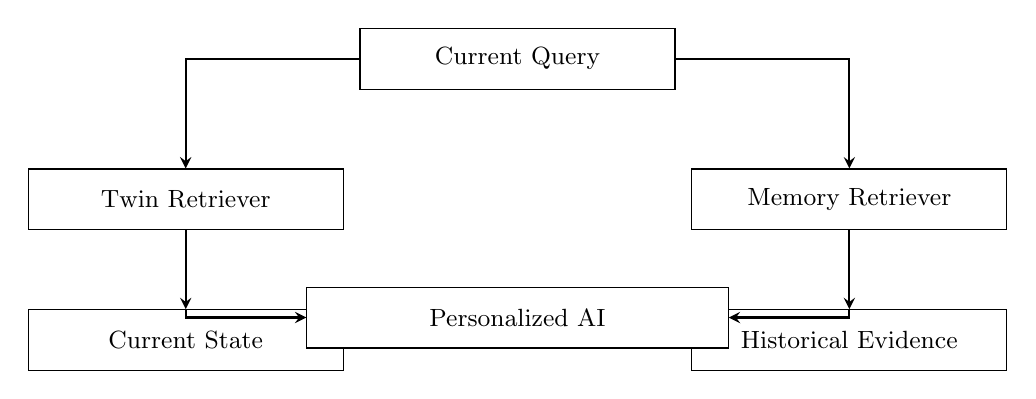
\begin{tikzpicture}[node distance=1cm and 1.5cm, auto]
    \node (query) [block] {Current Query};
    \node (twin_ret) [block, below left=1cm and 0.2cm of query, text width=3cm] {Twin Retriever};
    \node (mem_ret) [block, below right=1cm and 0.2cm of query, text width=3cm] {Memory Retriever};
    
    \node (state) [block, below=of twin_ret, text width=3cm] {Current State};
    \node (evidence) [block, below=of mem_ret, text width=3cm] {Historical Evidence};
    
    \node (ai) [block, below=2.5cm of query, text width=5cm] {Personalized AI};

    \draw [arrow] (query) -| (twin_ret);
    \draw [arrow] (query) -| (mem_ret);
    \draw [arrow] (twin_ret) -- (state);
    \draw [arrow] (mem_ret) -- (evidence);
    \draw [arrow] (state) |- (ai);
    \draw [arrow] (evidence) |- (ai);
\end{tikzpicture}
\caption{Retrieval Architecture.}
\end{figure}

This hybrid architecture allows the system to reason using both:
\begin{enumerate}[noitemsep,topsep=2pt]
    \item What the system currently believes about the learner
    \item Why the system believes it
\end{enumerate}

\section{Twin Retriever}
The \texttt{TwinRetriever} was designed to retrieve relevant learner information from the structured Digital Twin.

An important architectural challenge was identified during development.

Passing the entire Digital Twin to an LLM for every request can unnecessarily increase the context size and reduce efficiency.

The solution was to use hybrid retrieval.

Instead of always sending every learner attribute, the system retrieves the components relevant to the current request.

Certain relatively static information, such as profile and goals, can be injected directly when required, while dynamic components are retrieved selectively.

This significantly improves scalability and reduces unnecessary context.

\section{Twin Updater}
The Twin Updater is responsible for transforming new evidence into changes in the learner's current Digital Twin state.

The general pipeline is:
\begin{center}
\textbf{New Interaction} $\rightarrow$ \textbf{Evidence Extraction} $\rightarrow$ \textbf{Memory / Evidence} $\rightarrow$ \textbf{Affected Twin Components} $\rightarrow$ \textbf{Twin Update} $\rightarrow$ \textbf{Updated Learner State}
\end{center}

The key design principle is that the Twin represents the current state, while historical evidence remains in the Memory System.

This prevents the Digital Twin from becoming a large historical database.

\section{Current State vs Historical Evidence}
A major architectural decision in the project was the separation between current beliefs and historical evidence.

\paragraph{Digital Twin} Stores: \textit{``What do we currently believe about this learner?''}

\paragraph{Memory System} Stores: \textit{``What evidence have we observed that supports these beliefs?''}

This distinction is important for maintaining a clean and interpretable learner model.

For example:
\begin{itemize}[noitemsep,topsep=2pt]
    \item \textbf{Twin:} $\text{Python skill} = 0.80$
    \item \textbf{Memory:}
    \begin{itemize}[noitemsep,topsep=1pt]
        \item Completed Python project
        \item Reported confidence in Python
        \item Successfully solved programming task
        \item Previously struggled with advanced Python topics
    \end{itemize}
\end{itemize}

The Twin therefore remains compact while the evidence remains available when needed.

\section{Recommendation Engine}
The Recommendation Engine is intended to provide personalized suggestions based on the learner's current state.

Recommendations can consider:
\begin{itemize}[noitemsep,topsep=2pt]
    \item learner goals;
    \item current knowledge;
    \item skill levels;
    \item interests;
    \item preferences;
    \item historical memories;
    \item detected needs.
\end{itemize}

The objective is to avoid generic recommendations.

Instead of simply asking:
\begin{quote}
``What should a student learn?''
\end{quote}
the system can reason about:
\begin{quote}
``What should this particular student learn next given their goals, current knowledge, skills, preferences, and previous interactions?''
\end{quote}

\section{Prediction Engine}
The Prediction Engine is intended to use the learner model to make predictions about potential future outcomes or learning-related states.

Potential applications include:
\begin{itemize}[noitemsep,topsep=2pt]
    \item predicting areas where the learner may struggle;
    \item identifying skills requiring improvement;
    \item identifying learning priorities;
    \item estimating future learning needs;
    \item detecting gaps between current skills and desired goals.
\end{itemize}

The prediction component is designed to operate on the structured learner representation rather than treating every prediction as an isolated question.

\section{Explainability Module}
Explainability was incorporated to make AI decisions more understandable.

Personalized recommendations can be difficult to trust if the learner does not understand why they were generated.

The Explainability Module therefore provides a mechanism for connecting an output to the learner information and evidence that influenced it.

For example, a recommendation can be explained using factors such as:
\begin{itemize}[noitemsep,topsep=2pt]
    \item[] \textbf{Recommendation}
    \begin{itemize}[noitemsep,topsep=1pt]
        \item[$\vdash$] Learner Goal
        \item[$\vdash$] Current Skill
        \item[$\vdash$] Knowledge Gap
        \item[$\vdash$] Preference
        \item[$\llcorner$] Previous Evidence
    \end{itemize}
\end{itemize}

This makes the personalization process more transparent.

\section{AI Agents}
This section will be completed by the other team members responsible for the Agents component.

The final report will include the implementation and architecture of:
\begin{itemize}[noitemsep,topsep=2pt]
    \item AI Study Coach;
    \item AI Career Mentor;
    \item agent architecture;
    \item agent routing;
    \item agent workflows;
    \item tool usage;
    \item agent interaction with the Digital Twin;
    \item agent interaction with Memory Retrieval;
    \item agent interaction with Recommendation, Prediction, and Explainability modules.
\end{itemize}

Content to be added by the Agents team.

\section{Knowledge Graph}
This section will be completed by the other team members responsible for the Knowledge Graph component.

The final report will include:
\begin{itemize}[noitemsep,topsep=2pt]
    \item Knowledge Graph architecture;
    \item node and edge representation;
    \item knowledge relationships;
    \item graph construction;
    \item graph querying;
    \item graph integration with the Digital Twin;
    \item visualization;
    \item role of the Knowledge Graph in personalization and reasoning.
\end{itemize}

Content to be added by the Knowledge Graph team.

\section{Backend Architecture}
The backend was implemented as a Python-based service architecture.

The backend exposes the AI functionality through an API layer, allowing the frontend to communicate with the EduTwin system.

The general communication architecture is:
\begin{figure}[htbp]
\centering
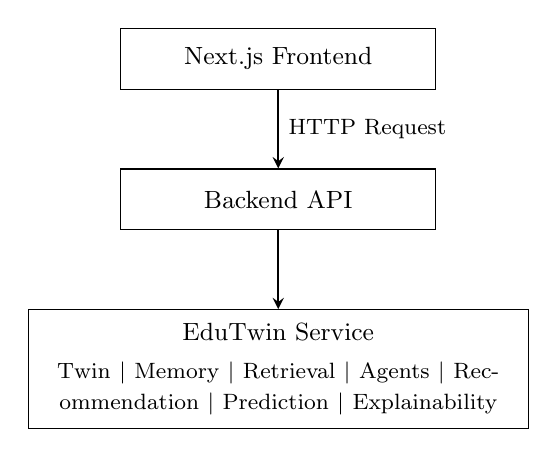
\begin{tikzpicture}[node distance=1cm, auto]
    \node (fe) [block] {Next.js Frontend};
    \node (api) [block, below=of fe] {Backend API};
    \node (srv) [block, below=of api, text width=6cm] {EduTwin Service\\[0.3em] \footnotesize Twin $\mid$ Memory $\mid$ Retrieval $\mid$ Agents $\mid$ Recommendation $\mid$ Prediction $\mid$ Explainability};

    \draw [arrow] (fe) -- node[right, font=\footnotesize] {HTTP Request} (api);
    \draw [arrow] (api) -- (srv);
\end{tikzpicture}
\caption{Backend Architecture Communication.}
\end{figure}

This separation keeps the frontend independent from the internal AI implementation.

\section{Service Layer}
A central EduTwin service was used to coordinate the system's functionality.

The service acts as an integration layer between the API and the underlying AI modules.

This allows a frontend request to pass through the system without requiring the frontend to understand the internal architecture.

For example:
\begin{center}
Frontend $\rightarrow$ /chat $\rightarrow$ EduTwin Service $\rightarrow$ Intent Detection $\rightarrow$ Relevant AI Capability $\rightarrow$ Twin + Memory Retrieval $\rightarrow$ LLM $\rightarrow$ Response
\end{center}

\section{Structured Data Models}
Pydantic-based models were used throughout the system to provide structured and validated data.

Models were developed for components including:
\begin{itemize}[noitemsep,topsep=2pt]
    \item Profile;
    \item Preferences;
    \item Knowledge;
    \item Skills;
    \item Memory;
    \item Memory Decision;
    \item Retrieval Request;
    \item Evidence;
    \item Student;
    \item Digital Twin components.
\end{itemize}

Using structured models helped maintain consistency between the different modules and reduced the risk of passing uncontrolled data between components.

\section{LLM Integration}
Large Language Models were used for tasks where natural-language understanding and structured reasoning were required.

The project used structured outputs where appropriate so that LLM results could be converted into validated application-level objects.

This was particularly important for the Memory Decision and learner-update processes.

Rather than relying entirely on free-form text, the system converts model outputs into structured representations that can be validated and processed programmatically.

\section{Error Handling and Integration Challenges}
Several integration challenges were encountered during implementation.

One issue involved storing Digital Twin component identifiers as metadata in ChromaDB.

The system initially attempted to store enumeration values directly in metadata, resulting in a metadata type error because ChromaDB expects supported primitive metadata values.

The issue was resolved by converting the affected component values into compatible representations before storage.

Another issue involved mixing timezone-aware and timezone-naive datetime objects during memory ranking.

The problem occurred when calculating recency because timestamps were represented using different timezone conventions.

The retrieval logic was corrected so that datetime comparisons use compatible representations.

These issues demonstrated the importance of validating data at the boundaries between independently developed components.

\section{Frontend / User Interface}
A major part of the final development stage was the creation of a modern web interface.

The frontend was implemented using:
\begin{itemize}[noitemsep,topsep=2pt]
    \item Next.js;
    \item TypeScript;
    \item Tailwind CSS.
\end{itemize}

The objective was not to create a simple research demonstration but a polished AI product interface.

\section{Unified Chat Experience}
The main interaction model is a single AI chat interface.

Instead of presenting separate pages for:
\begin{itemize}[noitemsep,topsep=2pt]
    \item Study Coach;
    \item Career Mentor;
    \item Recommendations;
    \item Prediction;
\end{itemize}
the learner interacts with one AI assistant.

The system internally determines the user's intent and activates the appropriate capability.

This creates a more natural experience:

\begin{figure}[htbp]
\centering
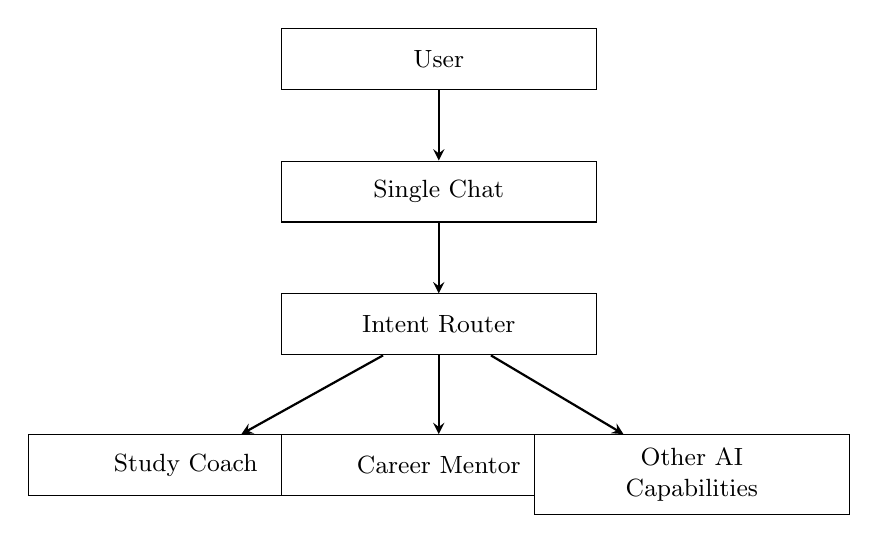
\begin{tikzpicture}[node distance=0.9cm, auto]
    \node (user) [block] {User};
    \node (chat) [block, below=of user] {Single Chat};
    \node (router) [block, below=of chat] {Intent Router};
    
    \node (coach) [block, below left=1cm and -0.8cm of router, text width=2.4cm] {Study Coach};
    \node (mentor) [block, below=1cm of router, text width=2.4cm] {Career Mentor};
    \node (other) [block, below right=1cm and -0.8cm of router, text width=2.4cm] {Other AI Capabilities};

    \draw [arrow] (user) -- (chat);
    \draw [arrow] (chat) -- (router);
    \draw [arrow] (router) -- (coach);
    \draw [arrow] (router) -- (mentor);
    \draw [arrow] (router) -- (other);
\end{tikzpicture}
\caption{Unified Chat Experience.}
\end{figure}

This design reduces cognitive load and avoids forcing the user to understand the internal architecture.

\section{Chat Interface}
The chat interface was implemented with dedicated components for:
\begin{itemize}[noitemsep,topsep=2pt]
    \item chat window;
    \item individual messages;
    \item message input;
    \item response rendering;
    \item automatic scrolling.
\end{itemize}

The interface was designed so that when the AI generates a new response, the conversation automatically moves toward the latest response, maintaining a natural conversational experience.

\section{User Interface Structure}
The planned application structure includes:

\paragraph{Chat} The primary interaction surface for communication with EduTwin.

\paragraph{My Twin / Profile} Displays the learner's current Digital Twin information.

\paragraph{Knowledge Graph} Provides a visual representation of relationships within the learner's knowledge representation.

\paragraph{Settings} Provides application-level configuration and user preferences.

The architecture intentionally avoids creating a separate page for every AI capability.

\section{Knowledge Graph Visualization}
The Knowledge Graph interface was developed as an interactive visualization rather than a static image.

The graph is intended to support:
\begin{itemize}[noitemsep,topsep=2pt]
    \item draggable nodes;
    \item visual relationships;
    \item interactive exploration;
    \item clearer representation of the learner's knowledge structure.
\end{itemize}

A dummy dataset was also used during GUI development to test the visualization before connecting it to the final knowledge representation.

This allowed the frontend design and interaction model to be developed independently from the final graph-generation pipeline.

Detailed Knowledge Graph implementation will be added by the responsible team members.

\section{Chat Persistence}
For the initial GUI implementation, conversation persistence was designed around browser-side storage.

\texttt{localStorage} was selected to avoid introducing unnecessary backend/database complexity during the development stage.

However, the conversation model and interfaces were designed so that the persistence layer can later be migrated to a real backend database when the application is prepared for production.

This provides a practical balance between rapid development and future scalability.

\section{Authentication and Application Structure}
The frontend architecture was also designed to support:
\begin{itemize}[noitemsep,topsep=2pt]
    \item login;
    \item signup;
    \item user-specific application state;
    \item profile access;
    \item settings;
    \item personalized Digital Twin information.
\end{itemize}

These components provide the foundation for turning the research prototype into a complete multi-user application.

\section{Technology Stack}
The project combines several technologies across the AI, backend, database, and frontend layers.

\begin{table}[htbp]
\centering
\renewcommand{\arraystretch}{1.2}
\begin{tabular}{|l|l|}
\hline
\textbf{Layer} & \textbf{Technology} \\
\hline
Frontend & Next.js \\
Frontend Language & TypeScript \\
Styling & Tailwind CSS \\
Backend & Python \\
API & FastAPI / Uvicorn \\
Data Validation & Pydantic \\
LLM & Gemini \\
Vector Database & ChromaDB \\
Embeddings & Vector embeddings \\
AI Architecture & Modular AI service architecture \\
Version Control & Git / GitHub \\
\hline
\end{tabular}
\caption{Technology Stack.}
\end{table}

The architecture was intentionally modular so that individual components can be replaced or improved independently.

\section{Software Architecture Principles}
Several principles guided the implementation.

\paragraph{Modularity} Each major function was separated into an independent component.

\paragraph{Structured Data} Pydantic models were used to define clear interfaces between components.

\paragraph{Separation of State and Evidence} The Digital Twin stores current beliefs while Memory stores historical evidence.

\paragraph{Retrieval-Based Context} Only relevant learner information is provided to the AI when possible.

\paragraph{Scalability} The architecture allows components such as the database, authentication layer, and memory persistence mechanism to be replaced or expanded later.

\paragraph{Explainability} The system attempts to retain information about why learner-related decisions are made.

\section{Hybrid Retrieval Strategy}
One of the important architectural outcomes of the project was the adoption of a hybrid retrieval strategy.

A purely static approach would pass the entire Digital Twin to the model.

A purely semantic approach would retrieve everything from a vector database.

Neither approach is ideal.

Instead, EduTwin combines:
\begin{center}
Static Learner Context $+$ Dynamic Twin Retrieval $+$ Historical Memory Retrieval
\end{center}

This provides the model with enough information to personalize the response without unnecessarily increasing the context size.

\section{Data Flow}
A typical user interaction can be described as follows:

\paragraph{Step 1 — User Interaction} The learner sends a message through the web interface.

\paragraph{Step 2 — API Request} The frontend sends the request to the backend API.

\paragraph{Step 3 — Intent Detection} The system determines what type of assistance is required.

\paragraph{Step 4 — Context Retrieval} Relevant information is retrieved from:
\begin{itemize}[noitemsep,topsep=2pt]
    \item Digital Twin;
    \item Memory System;
    \item other relevant system components.
\end{itemize}

\paragraph{Step 5 — AI Processing} The appropriate AI capability processes the request.

\paragraph{Step 6 — Response} A personalized response is returned to the frontend.

\paragraph{Step 7 — Evidence Extraction} The interaction is evaluated for potentially useful long-term information.

\paragraph{Step 8 — Memory} Meaningful evidence can be converted into a structured Memory object.

\paragraph{Step 9 — Twin Update} The learner model can be updated when new evidence changes the system's beliefs.

The overall lifecycle is:
\begin{center}
User $\rightarrow$ Interaction $\rightarrow$ Intent Detection $\rightarrow$ Retrieve Twin + Memories $\rightarrow$ AI Processing $\rightarrow$ Personalized Response $\rightarrow$ Evidence Detection $\rightarrow$ Memory $\rightarrow$ Twin Update $\rightarrow$ Updated Learner Model
\end{center}

\section{Testing and Debugging}
The system was tested progressively at both module and integration levels.

Testing included:
\begin{itemize}[noitemsep,topsep=2pt]
    \item memory creation;
    \item memory storage;
    \item duplicate detection;
    \item semantic retrieval;
    \item retrieval scoring;
    \item Digital Twin retrieval;
    \item service integration;
    \item backend API execution;
    \item frontend-backend communication;
    \item complete message processing.
\end{itemize}

The project also involved resolving integration errors between the vector database, Pydantic models, datetime handling, Gemini API integration, and the frontend API layer.

Testing the system through an independent service script before integrating it with the GUI was particularly useful because it allowed backend problems to be isolated from frontend problems.

\section{Development Workflow}
The project followed an iterative development process.

Initially, individual components were implemented independently.

These components were then integrated progressively:
\begin{center}
Data Models $\rightarrow$ Memory System $\rightarrow$ Memory Retrieval $\rightarrow$ Digital Twin Retrieval $\rightarrow$ Twin Updating $\rightarrow$ AI Services $\rightarrow$ Backend API $\rightarrow$ Frontend $\rightarrow$ Full System Integration
\end{center}

This approach allowed errors to be identified at the component level before the complete application was assembled.

\section{Research Contributions}
The project provides several contributions toward the development of personalized educational AI systems.

\subsection{Structured Learner Model}
The project demonstrates a structured approach to representing a learner using multiple Digital Twin components.

\subsection{Persistent Long-Term Memory}
The Memory System enables important evidence to persist beyond individual conversations.

\subsection{Separation of Current State and Evidence}
The architecture explicitly separates the learner's current beliefs from the historical evidence supporting those beliefs.

\subsection{Hybrid Retrieval}
The system combines current Digital Twin state with semantically retrieved historical memories.

\subsection{Dynamic Personalization}
The learner model can evolve as new interactions provide additional evidence.

\subsection{Unified AI Interface}
Multiple AI capabilities can be accessed through one conversational interface.

\subsection{Explainable Personalization}
The architecture provides a basis for explaining why particular recommendations or decisions were produced.

\section{Limitations}
Despite the progress achieved, several limitations remain.

\subsection{Dependence on LLM Quality}
Some learner-state decisions rely on LLM-generated structured outputs. Incorrect model judgments can therefore affect the Digital Twin.

\subsection{Limited Historical Validation}
A continuously evolving learner model requires evaluation over long periods to determine whether updates accurately reflect real learner development.

\subsection{Memory Quality}
Not every interaction provides meaningful evidence. The memory filtering and decision process therefore remains an important area for further improvement.

\subsection{Cold Start}
A new learner begins with limited information in their Digital Twin, reducing personalization during early interactions.

\subsection{Evaluation}
A major future requirement is a systematic experimental comparison between:
\begin{itemize}[noitemsep,topsep=2pt]
    \item a stateless AI assistant;
    \item an AI assistant with persistent memory;
    \item the complete Digital Twin architecture.
\end{itemize}

Such an experiment would provide stronger evidence for the project's central research question.

\section{Future Work}
Several extensions can be implemented in future versions.

\subsection{Production Database}
Browser \texttt{localStorage} can eventually be replaced by a persistent backend database for multi-device and multi-session synchronization.

\subsection{Improved Authentication}
A complete authentication and authorization system can be introduced for production deployment.

\subsection{Advanced Learner Modeling}
Future versions can introduce more sophisticated models for estimating knowledge mastery, skill development, and preference evolution.

\subsection{Temporal Twin Evolution}
The system can maintain more sophisticated temporal representations of learner development while preserving the separation between current state and historical evidence.

\subsection{Improved Recommendations}
Recommendation quality can be evaluated experimentally and improved using learner feedback.

\subsection{Automated Evaluation}
A dedicated evaluation framework can measure:
\begin{itemize}[noitemsep,topsep=2pt]
    \item personalization;
    \item relevance;
    \item recommendation quality;
    \item factual correctness;
    \item memory accuracy;
    \item learner satisfaction.
\end{itemize}

\subsection{Research Evaluation}
The most important future experiment is a controlled comparison between stateless and Digital-Twin-based AI systems.

Possible evaluation metrics include:
\begin{itemize}[noitemsep,topsep=2pt]
    \item relevance of responses;
    \item personalization score;
    \item recommendation usefulness;
    \item consistency;
    \item learner satisfaction;
    \item memory accuracy;
    \item adaptation over time.
\end{itemize}

\section{Conclusion}
EduTwin presents a modular architecture for an AI-powered Digital Twin designed specifically for education.

The project moves beyond the conventional stateless chatbot model by maintaining a structured and continuously evolving representation of the learner.

The Digital Twin represents current beliefs about the learner through components such as Profile, Goals, Preferences, Knowledge, Skills, and Interests. At the same time, the Memory System preserves historical evidence that can be retrieved when it becomes relevant.

A major architectural decision was to separate the current learner state from historical evidence. This keeps the Digital Twin compact while allowing the system to maintain long-term context.

The implementation also introduced semantic memory retrieval, hybrid Twin and Memory retrieval, structured LLM outputs, learner-state updating, recommendation and prediction capabilities, explainability, backend services, and a modern Next.js-based frontend.

The final GUI provides a unified conversational experience in which the learner interacts with one AI assistant while the system internally determines which capabilities are required.

The project therefore establishes the technical foundation for investigating the central research question:
\begin{quote}
\textit{Can a continuously evolving Digital Twin improve personalization compared with a stateless AI assistant?}
\end{quote}

While further empirical evaluation is required to answer this question conclusively, EduTwin demonstrates a complete architecture through which such an experiment can be conducted.

The project also provides a foundation for future development toward a production-ready personalized educational AI platform, with opportunities for stronger learner modeling, improved memory mechanisms, advanced knowledge representation, richer agent workflows, database-backed persistence, and quantitative evaluation.

\newpage
\appendix

\section{Main System Components}

\begin{table}[htbp]
\centering
\renewcommand{\arraystretch}{1.3}
\begin{tabular}{|l|p{9cm}|}
\hline
\textbf{Component} & \textbf{Main Responsibility} \\
\hline
Student & Aggregates the learner model \\
\hline
Profile & Stores relatively stable learner information \\
\hline
Goals & Represents learner objectives \\
\hline
Preferences & Represents learner preference beliefs \\
\hline
Knowledge & Represents current knowledge/mastery beliefs \\
\hline
Skills & Represents skill level and confidence \\
\hline
Memory & Stores historical learner evidence \\
\hline
Memory Store & Persists memories using ChromaDB \\
\hline
Memory Retriever & Retrieves relevant historical evidence \\
\hline
Twin Retriever & Retrieves relevant learner-state information \\
\hline
Twin Updater & Updates current Digital Twin beliefs \\
\hline
Recommendation Engine & Generates personalized recommendations \\
\hline
Prediction Engine & Produces learner-related predictions \\
\hline
Explainability Module & Explains AI decisions \\
\hline
Agents & Provides specialized AI capabilities \\
\hline
Knowledge Graph & Represents relationships within learner knowledge \\
\hline
Backend API & Connects frontend and AI services \\
\hline
Frontend & Provides the learner-facing application \\
\hline
\end{tabular}
\caption{Main System Components.}
\end{table}

\newpage
\section{Key Architectural Principle}
The central design principle of EduTwin can be summarized as:

\begin{figure}[htbp]
\centering
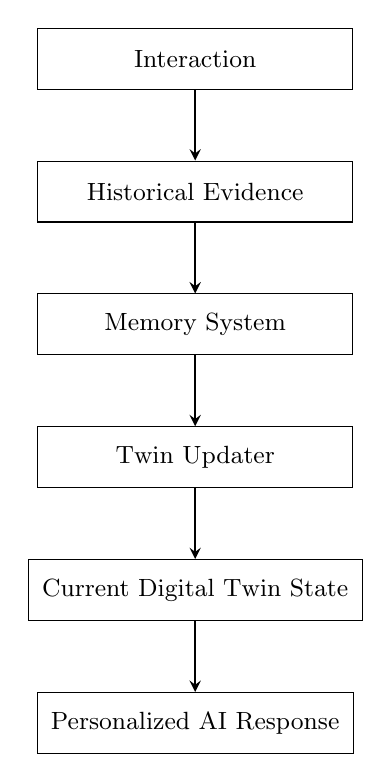
\begin{tikzpicture}[node distance=0.9cm, auto]
    \node (interaction) [block] {Interaction};
    \node (evidence) [block, below=of interaction] {Historical Evidence};
    \node (memory) [block, below=of evidence] {Memory System};
    \node (updater) [block, below=of memory] {Twin Updater};
    \node (twin) [block, below=of updater] {Current Digital Twin State};
    \node (ai) [block, below=of twin] {Personalized AI Response};

    \draw [arrow] (interaction) -- (evidence);
    \draw [arrow] (evidence) -- (memory);
    \draw [arrow] (memory) -- (updater);
    \draw [arrow] (updater) -- (twin);
    \draw [arrow] (twin) -- (ai);
\end{tikzpicture}
\caption{Key Architectural Principle Flow.}
\end{figure}

The Digital Twin answers:
\begin{quote}
``What do we currently believe about the learner?''
\end{quote}
while the Memory System answers:
\begin{quote}
``What evidence do we have about the learner?''
\end{quote}

Together, these two layers form the foundation of EduTwin's personalization architecture.

\end{document}
